%%%%%%%%%%%%%%%%%%%%%%%%%%%%%%%%%%%%
% Slide options
%%%%%%%%%%%%%%%%%%%%%%%%%%%%%%%%%%%%

% Option 1: Slides with solutions

\documentclass[slidestop,compress,mathserif]{beamer}
\usepackage{pgfplots}
\usetikzlibrary{positioning}
\usepackage{booktabs}
\newcommand{\soln}[1]{\textit{#1}}
\newcommand{\solnGr}[1]{#1}

% Option 2: Handouts without solutions

%\documentclass[11pt,containsverbatim,handout]{beamer}
%\usepackage{pgfpages}
%\pgfpagesuselayout{4 on 1}[letterpaper,landscape,border shrink=5mm]
%\newcommand{\soln}[1]{ }
%\newcommand{\solnGr}{ }

%%%%%%%%%%%%%%%%%%%%%%%%%%%%%%%%%%%%
% Style
%%%%%%%%%%%%%%%%%%%%%%%%%%%%%%%%%%%%
%%%%%%%%%%%%%%%%%%%%%%%%%%%%%%%%%%%%%%%%%%%%%%%%%%%%%%%%%%%%%%%%%%%%%%%%
% MA213/214 shared slide style
%
% "Calm & Cool" palette + content-type callout boxes.
% Overhauled (2026) from the original OpenIntro/metropolis style:
%   - all OpenIntro visual branding removed (logo, grid, colors)
%   - a low-key cool palette (see colors below)
%   - tcolorbox callout boxes so students recognize content types
% See common/README.md for the command cheat-sheet.
%%%%%%%%%%%%%%%%%%%%%%%%%%%%%%%%%%%%%%%%%%%%%%%%%%%%%%%%%%%%%%%%%%%%%%%%

\usetheme{metropolis}

%%%%%%%%%%%%%%%%
% Packages
%%%%%%%%%%%%%%%%

\usepackage{geometry}
\usepackage{graphicx}
\usepackage{amssymb}
\usepackage{epstopdf}
\usepackage{amsmath}  	% this permits text in eqnarray among other benefits
\usepackage{url}		% produces hyperlinks
\usepackage{hyperref}	% allows for color usage in tables
\usepackage[english]{babel}
\usepackage[latin1]{inputenc}
\usepackage{colortbl}	% allows for color usage in tables
\usepackage{multirow}	% allows for rows that span multiple rows in tables
\usepackage{color}		% this package has a variety of color options
\usepackage{pgf}
\usepackage{calc}
\usepackage{ulem}
\usepackage{multicol}
\usepackage{textcomp}
\usepackage{txfonts}
\usepackage{listings}
\usepackage{tikz}
\usepackage{array}
\usepackage{wasysym}
\usepackage{fancyvrb}
\usepackage{etoolbox}             % \ifstrempty for optional box subtitles
\usepackage[most]{tcolorbox}      % content-type callout boxes
\tcbuselibrary{listings}          % R-code block (\begin{rblock})
\usepackage{fontawesome5}         % box icons

%%%%%%%%%%%%%%%%
% Remove navigation symbols
%%%%%%%%%%%%%%%%

\setbeamertemplate{navigation symbols}{}

%%%%%%%%%%%%%%%%
% "Calm & Cool" palette
%%%%%%%%%%%%%%%%

% chrome / structure / body
\definecolor{ccSlate}{HTML}{2E3742}   % frametitle bar, structure, section pages (deep neutral slate)
\definecolor{ccInk}{HTML}{2B2B2B}     % body text
\definecolor{ccWash}{HTML}{FCF8F1}    % gentle warm title-slide background wash (complements the cool blues)

% example (blue)
\definecolor{ccBlue}{HTML}{2F6690}
\definecolor{ccBlueBg}{HTML}{EAF1F7}
% interactive activity / discussion (green)
\definecolor{ccGreen}{HTML}{4E8A6B}
\definecolor{ccGreenBg}{HTML}{E9F3EC}
% solution (purple)
\definecolor{ccPurple}{HTML}{6F5499}
\definecolor{ccPurpleBg}{HTML}{EFEAF6}
% worksheet / focused work (terracotta)
\definecolor{ccTerra}{HTML}{C2693E}
\definecolor{ccTerraBg}{HTML}{FAEDE4}
% formula / definition (neutral slate)
\definecolor{ccGray}{HTML}{5C6B7A}
\definecolor{ccGrayBg}{HTML}{EEF1F4}
% caution / common pitfall (brick red)
\definecolor{ccRed}{HTML}{B23A48}
\definecolor{ccRedBg}{HTML}{FAEAEC}
% key idea / takeaway (muted gold)
\definecolor{ccGold}{HTML}{9C7A28}
\definecolor{ccGoldBg}{HTML}{F7F1DF}
% learning goals / lesson outcomes (teal)
\definecolor{ccTeal}{HTML}{2C6E6B}
\definecolor{ccTealBg}{HTML}{E6F0EF}
% learning objectives (indigo)
\definecolor{ccIndigo}{HTML}{45507A}
\definecolor{ccIndigoBg}{HTML}{ECEEF4}
% R code / output (gray)
\definecolor{ccCode}{HTML}{5F5E5A}
\definecolor{ccCodeBg}{HTML}{F4F5F6}

% neutral grays kept from the original style
\definecolor{gray}{rgb}{0.5, 0.5, 0.5}
\definecolor{darkGray}{rgb}{0.3, 0.3, 0.3}
\definecolor{darkerGray}{rgb}{0.2, 0.2, 0.2}

% Backwards-compatible aliases: old OpenIntro color names now point at the
% new palette, so existing \textcolor{oiB}{...}, \hl{...}, etc. keep working.
\colorlet{oiB}{ccBlue}
\colorlet{oiG}{ccGreen}
\colorlet{hlblue}{ccBlue}
\colorlet{rubineRed}{ccRed}
\colorlet{irishGreen}{ccGreen}
\colorlet{lightGreen}{ccGreen}

%%%%%%%%%%%%%%%%
% Restyle metropolis with the Calm & Cool chrome
%%%%%%%%%%%%%%%%

\metroset{block=fill}

\setbeamercolor{normal text}{fg=ccInk, bg=white}
\setbeamercolor{structure}{fg=ccSlate}
\setbeamercolor{alerted text}{fg=ccBlue}
\setbeamercolor{example text}{fg=ccGreen}
\setbeamercolor{frametitle}{bg=ccSlate, fg=white}
\setbeamercolor{progress bar}{fg=ccBlue}
\setbeamercolor{title separator}{fg=ccBlue}
\setbeamercolor{title}{fg=ccSlate}
\setbeamercolor{subtitle}{fg=ccBlue}
\setbeamercolor{author}{fg=ccInk}
\setbeamercolor{institute}{fg=ccGray}
\setbeamercolor{date}{fg=ccGray}
\setbeamercolor{section title}{fg=ccSlate}
\setbeamercolor{standout}{fg=white, bg=ccSlate}

% Section pages sit on the same warm wash as the title slide. We keep
% metropolis's section-title styling and just paint a full-page ccWash
% background behind it (needs >=2 pdflatex passes for the current-page node).
\setbeamertemplate{section page}{%
  \begin{tikzpicture}[remember picture, overlay]
    \fill[ccWash] (current page.south west) rectangle (current page.north east);
  \end{tikzpicture}%
  \centering
  \begin{minipage}{22em}
    \raggedright
    \usebeamercolor[fg]{section title}%
    \usebeamerfont{section title}%
    \insertsectionhead\\[-1ex]
    \usebeamertemplate*{progress bar in section page}%
    \par
  \end{minipage}\par
  \vspace{\baselineskip}
}

%%%%%%%%%%%%%%%%
% Custom inline text commands (recolored to the palette)
%%%%%%%%%%%%%%%%

% degree
\newcommand{\degree}{\ensuremath{^\circ}}

% cite
\newcommand{\ct}[1]{
\vfill
{\tiny #1}}

\newcommand{\NamedNote}[2]{
\rule{2.5cm}{0.25pt} \\ \textit{\footnotesize{\textcolor{rubineRed}{#1:} \textcolor{darkerGray}{#2}}}}

% Note
\newcommand{\Note}[1]{
\rule{2.5cm}{0.25pt} \\ \textit{\footnotesize{\textcolor{rubineRed}{Note:} \textcolor{darkerGray}{#1}}}}

% Remember
\newcommand{\Remember}[1]{\textit{\scriptsize{\textcolor{ccTerra}{Remember:} #1}}}

% expected counts
\newcommand{\ex}[1]{\textit{\textcolor{ccBlue}{#1}}}

% red
\newcommand{\red}[1]{\textit{\textcolor{rubineRed}{#1}}}

% pink
\newcommand{\pink}[1]{\textit{\textcolor{rubineRed!90!white!50}{#1}}}

% green
\newcommand{\green}[1]{\textit{\textcolor{irishGreen}{#1}}}

% orange
\newcommand{\orange}[1]{\textit{\textcolor{ccTerra}{#1}}}

% links: webURL, webLink, appLink
\newcommand{\webURL}[1]{\urlstyle{same}{ \textit{\textcolor{darkGray}{\url{#1}}}}}
\newcommand{\webLink}[2]{\href{#1}{\textcolor{darkGray}{{#2}}}}
\newcommand{\appLink}[2]{\href{#1}{\textcolor{white}{{#2}}}}

% mail
\newcommand{\mail}[1]{\href{mailto:#1}{\textit{\textcolor{darkGray}{#1}}}}

% highlighting: hl, hlGr, mathhl
\newcommand{\hl}[1]{\textit{\textcolor{hlblue}{#1}}}
\newcommand{\hlGr}[1]{\textit{\textcolor{lightGreen}{#1}}}
\newcommand{\mathhl}[1]{\textcolor{hlblue}{\ensuremath{#1}}}

%%%%%%%%%%%%%%%%
% Structural helpers (unchanged from the original)
%%%%%%%%%%%%%%%%

% two col: two columns
\newenvironment{twocol}[4]{
\begin{columns}[c]
\column{#1\textwidth}
#3
\column{#2\textwidth}
#4
\end{columns}
}

% slot (for probability calculations)
\newenvironment{slot}[2]{
\begin{array}{c}
\underline{#1} \\
#2
\end{array}
}

% pr: left and right parentheses
\newcommand{\pr}[1]{
\left( #1 \right)
}

% cancel
\newcommand{\cancel}[1]{%
    \tikz[baseline=(tocancel.base)]{
        \node[inner sep=0pt,outer sep=0pt] (tocancel) {#1};
        \draw[red, line width=0.5mm] (tocancel.south west) -- (tocancel.north east);
    }%
}

% removepagenumbers
\newcommand{\removepagenumbers}{%
  \setbeamertemplate{footline}{}
}

% change margin
\newenvironment{changemargin}[2]{%
\begin{list}{}{%
\setlength{\topsep}{0pt}%
\setlength{\leftmargin}{#1}%
\setlength{\rightmargin}{#2}%
\setlength{\listparindent}{\parindent}%
\setlength{\itemindent}{\parindent}%
\setlength{\parsep}{\parskip}%
}%
\item}{\end{list}}

% footnote
\long\def\symbolfootnote[#1]#2{\begingroup%
\def\thefootnote{\fnsymbol{footnote}}\footnote[#1]{#2}\endgroup}

% commands from the book
\newenvironment{data}[1]{\texttt{#1}}{}
\newenvironment{var}[1]{\texttt{#1}}{}
\newenvironment{resp}[1]{\texttt{#1}}{}

%%%%%%%%%%%%%%%%
% Content-type callout boxes (tcolorbox)
%
% Each type has a colored title strip (icon + label) over a light fill.
% Color = content type; the label + icon reinforce it (so the cue does
% not rely on color alone).
%%%%%%%%%%%%%%%%

\tcbset{
  cccallout/.style 2 args={
    enhanced, breakable=false,
    colback=#2, colframe=#1, colbacktitle=#1, coltitle=white,
    fonttitle=\bfseries\footnotesize,
    boxrule=0.6pt, arc=2.5pt, outer arc=2.5pt,
    left=5pt, right=5pt, top=3pt, bottom=3pt, boxsep=2pt,
    toptitle=2pt, bottomtitle=2pt, lefttitle=5pt,
    before skip=5pt, after skip=5pt,
  },
}

% One-off / collection of examples (blue): \workedexample[subtitle]{body}.
% (Named \workedexample, not \example, because beamer defines \example.)
\newtcolorbox{examplebox}[1][]{cccallout={ccBlue}{ccBlueBg},
  title={\faIcon{lightbulb}~~Example\ifstrempty{#1}{}{ \textmd{---}\ #1}}}
\newcommand{\workedexample}[2][]{\begin{examplebox}[#1]#2\end{examplebox}}

% Running-example header (blue): \examplehead{name} at the top of each frame of a
% multi-slide running example. A one-off or a collection of examples uses the
% \workedexample box above instead.
\newcommand{\examplehead}[1]{%
  \vspace{-0.4em}\par\noindent\tcbox[on line, colback=ccBlue, colframe=ccBlue, coltext=white,
    boxrule=0pt, arc=2pt, left=5pt, right=5pt, top=1pt, bottom=1pt,
    box align=base, nobeforeafter]{\footnotesize\bfseries\faIcon{lightbulb}\,Running example}%
  \ifstrempty{#1}{}{\enspace{\footnotesize\bfseries\textcolor{ccBlue}{#1}}}%
  \par\nobreak\vspace{-0.6em}{\color{ccBlue}\rule{\linewidth}{0.7pt}}\par\nobreak\vspace{-0.8em}}

% Interactive activity (green): \activity[subtitle]{body}
\newtcolorbox{activitybox}[1][]{cccallout={ccGreen}{ccGreenBg},
  title={\faIcon{users}~~Activity\ifstrempty{#1}{}{ #1}}}
\newcommand{\activity}[2][]{\begin{activitybox}[#1]#2\end{activitybox}}

% Discussion question (green): \dq{body}
\newtcolorbox{dqbox}{cccallout={ccGreen}{ccGreenBg}, title={\faIcon{comments}~~Discussion}}
\newcommand{\dq}[1]{\begin{dqbox}#1\end{dqbox}}

% Solution (purple): \solnbox{body}. Gated by the per-deck \soln toggle, so it
% shows in the instructor build and vanishes from the student handout build.
% (Named \solnbox, not \solution, because beamer already defines \solution.)
\newtcolorbox{solutionbox}{cccallout={ccPurple}{ccPurpleBg}, title={\faIcon{key}~~Solution}}
\newcommand{\solnbox}[1]{\soln{\begin{solutionbox}#1\end{solutionbox}}}

% Worksheet / focused work (terracotta): \worksheet[subtitle]{body}
\newtcolorbox{worksheetbox}[1][]{cccallout={ccTerra}{ccTerraBg},
  title={\faIcon{pencil-alt}~~Worksheet\ifstrempty{#1}{}{ #1}}}
\newcommand{\worksheet}[2][]{\begin{worksheetbox}[#1]#2\end{worksheetbox}}

% Formula / definition (neutral slate). Supports both real usages found in the
% decks: \formula{title}{body} and the bare \formula{body} (title defaults to
% "Formula"). The second group is an optional brace argument.
\newtcolorbox{formulabox}[1][Formula]{cccallout={ccGray}{ccGrayBg},
  title={\faIcon{square-root-alt}~~#1}}
\NewDocumentCommand{\formula}{m g}{%
  \IfNoValueTF{#2}%
    {\begin{formulabox}#1\end{formulabox}}%
    {\begin{formulabox}[#1]#2\end{formulabox}}}

% Common pitfall / caution (brick red): \caution[subtitle]{body}
\newtcolorbox{cautionbox}[1][]{cccallout={ccRed}{ccRedBg},
  title={\faIcon{exclamation-triangle}~~Caution\ifstrempty{#1}{}{ #1}}}
\newcommand{\caution}[2][]{\begin{cautionbox}[#1]#2\end{cautionbox}}

% Key idea / takeaway (muted gold): \keyidea[subtitle]{body}
\newtcolorbox{keyideabox}[1][]{cccallout={ccGold}{ccGoldBg},
  title={\faIcon{star}~~Key idea\ifstrempty{#1}{}{ #1}}}
\newcommand{\keyidea}[2][]{\begin{keyideabox}[#1]#2\end{keyideabox}}

% Learning goals / lesson outcomes (teal): \goals{body}. Sits under the short
% LO headings on the objectives slide; body is the "you should be able to" list.
\newtcolorbox{goalsbox}{cccallout={ccTeal}{ccTealBg}, fontupper=\footnotesize,
  top=1pt, bottom=2pt, boxsep=1pt, before skip=3pt,
  title={\faIcon{bullseye}~~By the end of today, you should be able to\ldots}}
\newcommand{\goals}[1]{\begin{goalsbox}#1\end{goalsbox}}

% Learning objectives (indigo): \objectives{body} -- the formal LO headings,
% shown alongside \goals on the objectives slide.
\newtcolorbox{objectivesbox}{cccallout={ccIndigo}{ccIndigoBg}, fontupper=\small,
  top=1pt, bottom=2pt, boxsep=1pt, before skip=3pt,
  title={\faIcon{clipboard-list}~~Learning objectives}}
\newcommand{\objectives}[1]{\begin{objectivesbox}#1\end{objectivesbox}}

% Defaults for a bare \begin{lstlisting}. Without these it inherits the listings
% package defaults: 11pt type, fixed-width columns (which spaces code out as
% "a g e _ f i t"), and no line breaking, so a long line silently runs off the
% right edge of the slide. A deck that passes its own basicstyle still wins.
% Layout only -- syntax coloring is left to the \begin{rblock} environment.
\lstset{
  basicstyle=\ttfamily\footnotesize, columns=fullflexible,
  breaklines=true, breakindent=1.5em, showstringspaces=false,
  numbers=none, frame=none}

% R code / output (gray): \begin{rblock}[subtitle] ... \end{rblock}
% NOTE: a frame containing an rblock must be declared \begin{frame}[fragile].
\lstdefinestyle{ccR}{
  language=R, basicstyle=\ttfamily\footnotesize, columns=fullflexible,
  breaklines=true, showstringspaces=false, numbers=none, frame=none,
  keywordstyle=\color{ccBlue}, commentstyle=\color{ccGreen!75!black},
  stringstyle=\color{ccTerra}}
\newtcblisting{rblock}[1][]{cccallout={ccCode}{ccCodeBg},
  title={\faIcon{terminal}~~R\ifstrempty{#1}{}{ #1}},
  listing only, listing style=ccR}

% --- Legacy boxes (kept so existing decks compile) ---

% app: application exercise -> alias of activity
\newcommand{\app}[1]{\activity{#1}}

% pq: practice question (green, interactive family)
\newtcolorbox{pqbox}{cccallout={ccGreen}{ccGreenBg}, title={\faIcon{list-ol}~~Practice}}
\newcommand{\pq}[1]{\begin{pqbox}#1\end{pqbox}}

% solnMult: solutions for multiple-choice practice questions (uses \soln toggle)
\newcommand{\solnMult}[1]{
\item[] \vspace{-0.59cm}
\only<1>{\item #1}
\soln{\only<2->{\item \orange{#1}}}
}

%%%%%%%%%%%%%%%%
% De-branded title frame + attribution
%%%%%%%%%%%%%%%%

% Eyebrow line on the title slide; a deck may \renewcommand this.
\newcommand{\coursetag}{MA214: Applied Statistics}

% Attribution: all slides released under CC BY-SA, crediting both the
% instructor (later material) and OpenIntro (basis of the earlier material).
\newcommand{\courseattribution}{%
  Slides by Jonathan H.~Huggins, building on materials from OpenIntro's
  \emph{Introduction to Modern Statistics} (Mine \c{C}etinkaya-Rundel et al.).
  Released under the
  \webLink{http://creativecommons.org/licenses/by-sa/3.0/us/}{CC BY-SA license}.
  Some images included under fair use (educational purposes).}

% \maketitleframe: de-branded title slide (no logo, no grid). Uses the deck's
% \title, \subtitle, and \coursetag.
\newcommand{\maketitleframe}{%
  \addtocounter{framenumber}{-1}%
  {\removepagenumbers
  \setbeamercolor{background canvas}{bg=ccWash}%
  \begin{frame}[plain]
    \vspace*{2.6em}
    {\color{ccSlate}\rule{\textwidth}{2.5pt}}\par\vspace{1.5em}
    {\usebeamerfont{date}\scshape\color{ccGray}\coursetag}\par\vspace{0.55em}
    {\usebeamerfont{title}\color{ccSlate}\inserttitle\par}
    \vspace{0.45em}{\color{ccBlue}\rule{3em}{2.5pt}}\par\vspace{0.7em}
    {\usebeamerfont{subtitle}\color{ccBlue}\insertsubtitle\par}
    \vfill
    {\color{ccGray!55}\rule{\textwidth}{0.4pt}}\par\vspace{0.45em}
    {\tiny\color{ccGray}\courseattribution\par}
    \vspace*{0.4em}
  \end{frame}}}

%%%%%%%%%%%%%%%%
% Graphics
%%%%%%%%%%%%%%%%

\DeclareGraphicsRule{.tif}{png}{.png}{`convert #1 `dirname #1`/`basename #1 .tif`.png}

\graphicspath{ {../../common/} {figures/}  }


%%%%%%%%%%%%%%%%%%%%%%%%%%%%%%%%%%%%
% Preamble
%%%%%%%%%%%%%%%%%%%%%%%%%%%%%%%%%%%%

\title[Lecture 9]{Lecture 9: Confidence intervals with bootstrapping}
\subtitle{Module 2: Statistical Inference}
\author{Introduction to Modern Statistics, 2nd Edition}
\institute{$\:$ \\ {\footnotesize Based on slides developed by Mine \c{C}etinkaya-Rundel of OpenIntro.  \\
The slides may be copied, edited, and/or shared via the \webLink{http://creativecommons.org/licenses/by-sa/3.0/us/}{CC BY-SA license.} \\
Some images may be included under fair use guidelines (educational purposes).}}
\date{}

%%%%%%%%%%%%%%%%%%%%%%%%%%%%%%%%%%%%
% Begin document
%%%%%%%%%%%%%%%%%%%%%%%%%%%%%%%%%%%%

\begin{document}


%%%%%%%%%%%%%%%%%%%%%%%%%%%%%%%%%%%%
% Title page
%%%%%%%%%%%%%%%%%%%%%%%%%%%%%%%%%%%%

\maketitleframe

% !TEX root =  Lecture10.tex


%%%%%%%%%%%%%%%%%%%%%%%%%%%%%%%%%%%%
% Recap/Agenda
%%%%%%%%%%%%%%%%%%%%%%%%%%%%%%%%%%%%
\begin{frame}
\frametitle{Module 2: Statistical Inference}
    \begin{itemize}
    	\item \hl{Previously:} testing with randomization --- \emph{is there an effect?}
        \item \hl{This time:} \emph{how big is it?} Confidence intervals with bootstrapping.
          \begin{itemize}
              \item confidence intervals as statements about a \emph{procedure};
              \item the bootstrap idea: resample your own data with replacement;
              \item percentile and standard-error intervals, and what makes them narrow;
              \item doing it in R --- and what the bootstrap cannot do.
          \end{itemize}
        \item \hl{Reading:} IMS Chapter 12.
        \item \hl{Homework for today:}
        \item \hl{Homework for next class:}
    \end{itemize}
\end{frame}


%%%%%%%%%%%%%%%%%%%%%%%%%%%%%%%%%%%%
% Learning objectives:
%%%%%%%%%%%%%%%%%%%%%%%%%%%%%%%%%%%%
\begin{frame}
    \frametitle{Lecture Objectives}
    \goals{%
    \begin{itemize}
    \item say what population \emph{parameter} a scientific question is really asking about;
    \item build a bootstrap distribution --- resample, recompute, repeat --- and read a confidence interval off it, by percentile or by standard error;
    \item interpret a confidence interval correctly, and name the three standard misreadings;
    \item carry the whole workflow out in R, and choose between randomization, bootstrapping, and a mathematical model.
    \end{itemize}}
    \objectives{%
    \begin{itemize}
    \item \textbf{(M2, LO1)} Approaches to Inference
    \item \textbf{(M2, LO2)} Simulation-based Inference
    \end{itemize}}
\end{frame}


%%%%%%%%%%%%%%%%%%%%%%%%%%%%%%%%%%%%%%%%%%%%%%%%%%%%%%%%%%%%%%%%%%%%%%%%
\section{From testing to estimation}
%%%%%%%%%%%%%%%%%%%%%%%%%%%%%%%%%%%%%%%%%%%%%%%%%%%%%%%%%%%%%%%%%%%%%%%%
\begin{frame}
\frametitle{From ``Is there an effect?'' to ``How big is it?''}

\begin{itemize}
\item Last time, hypothesis tests and p-values were about \textbf{evidence against a null model}.
\item Today, assuming we have a reasonable statistic, we ask how \textbf{reliable} the estimate is.
\item The question we use to assess reliability is:
\end{itemize}

\vspace{0.5em}
\begin{center}
\Large \hl{If we repeated the study, how much would our estimate change?}
\end{center}

\vspace{0.5em}
This is about a \textbf{sampling distribution}, or an approximation to it.

\end{frame}

%%%%%%%%%%%%%%%%%%%%%%%%%%%%%%%%%%%%%%%%%%%%%%%%%%%%%%%%%%%%%%%%%%%%%%%%

\begin{frame}
\frametitle{Inference workflow: where bootstrapping fits}

\keyidea[-- the road to an interval]{
\begin{center}
Question $\Rightarrow$ parameter $\Rightarrow$ statistic $\Rightarrow$ sampling distribution $\Rightarrow$ interval
\end{center}}

\vspace{0.2em}
{\small
\begin{itemize}
\item \hl{Parameter:} unknown population quantity, such as $\mu$, $p$, or $\mu_1-\mu_2$.
\item \hl{Statistic:} value computed from the sample, such as $\bar{x}$, $\hat{p}$, or $\bar{x}_1-\bar{x}_2$.
\item \hl{Sampling distribution:} how the statistic varies across repeated samples; this, not the spread of the raw data, is the uncertainty a confidence interval is built around.
\item \hl{Bootstrap distribution:} a simulation-based approximation to that sampling distribution, and the only one of the four we can actually compute today.
\end{itemize}}

\end{frame}

%%%%%%%%%%%%%%%%%%%%%%%%%%%%%%%%%%%%%%%%%%%%%%%%%%%%%%%%%%%%%%%%%%%%%%%%
\section{The parameter of interest}
%%%%%%%%%%%%%%%%%%%%%%%%%%%%%%%%%%%%%%%%%%%%%%%%%%%%%%%%%%%%%%%%%%%%%%%%
\begin{frame}
\frametitle{A running example: kangaroo rats}
\examplehead{Kangaroo rats}
\textbf{Data.} Captures from the \webLink{https://portal.weecology.org/}{Portal Project} near Portal, Arizona; the $n=348$ kangaroo rats weighed in 1999.

\textbf{Question.} What is a typical body mass, and how sure can we be from this \emph{one} sample?
\begin{center}
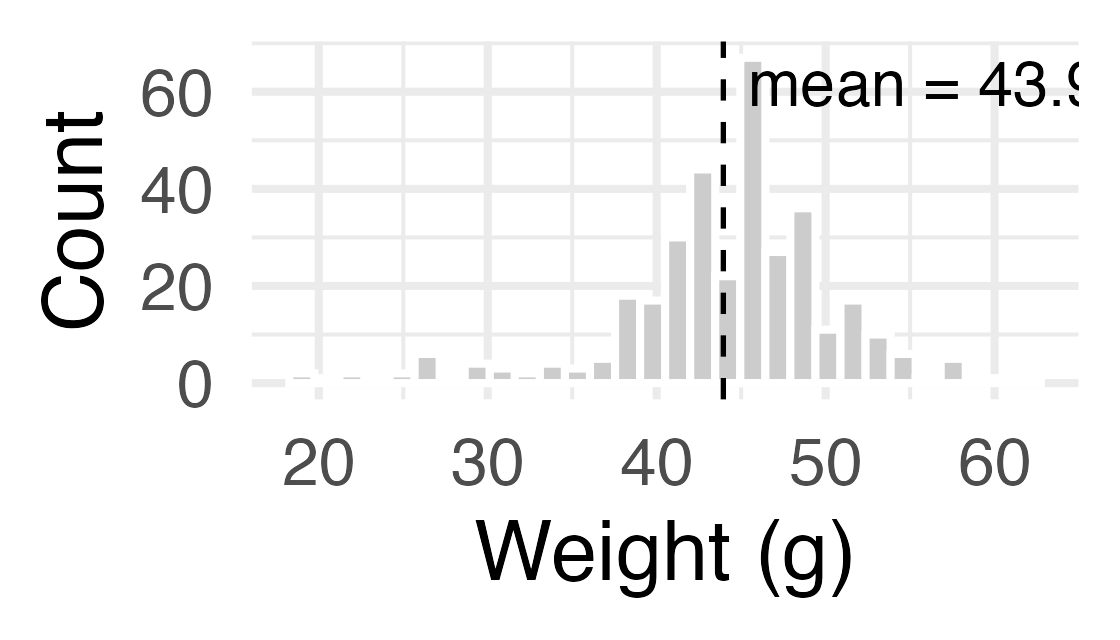
\includegraphics[width=0.42\textwidth]{dm1999_hist.png}
\end{center}

\end{frame}

%%%%%%%%%%%%%%%%%%%%%%%%%%%%%%%%%%%%%%%%%%%%%%%%%%%%%%%%%%%%%%%%%%%%%%%%
\begin{frame}
\frametitle{Parameters of interest}

Let $X$ be the weight in grams of a randomly selected kangaroo rat from the population.

\vspace{0.1em}
\begin{center}\scriptsize\setlength{\tabcolsep}{4pt}
\begin{tabular}{lll}
\toprule
Parameter & Sample statistic & Answers the question \\
\midrule
$\mu = E[X]$ & $\bar{x}$ & average mass; biomass and energy budgets \\
$m = \mathrm{median}(X)$ & sample median & the typical individual (robust to skew) \\
$q_{0.10}$ & sample 10th percentile & how small the small ones are \\
$q_{0.90}$ & sample 90th percentile & how big the big ones get; predation thresholds \\
\bottomrule
\end{tabular}
\end{center}

\vspace{0.1em}
\dq{Different parameters answer different questions, so what exactly is the \emph{population} here? All kangaroo rats at this site in 1999? In the desert? Ever?}

\end{frame}

%%%%%%%%%%%%%%%%%%%%%%%%%%%%%%%%%%%%%%%%%%%%%%%%%%%%%%%%%%%%%%%%%%%%%%%%

\begin{frame}
\frametitle{Activity: parameter, statistic, or raw data?}

For each phrase, decide whether it describes a parameter, a statistic, or raw data.

\app{
\begin{enumerate}
\item The mean weight of all kangaroo rats in the study population.
\item The mean weight of the kangaroo rats in our sample.
\item The list of observed weights: $44, 46, 42, 51, \ldots$.
\item The median weight of all kangaroo rats in the population.
\item The bootstrap means produced after 2000 resamples.
\end{enumerate}}

\pause
\vspace{-0.4em}
{\footnotesize
\soln{(1) parameter ($\mu$). (2) statistic ($\bar{x}$). (3) raw data. (4) parameter ($m$). (5) 2000 \emph{statistics}, one per resample. That last one is the whole point: a bootstrap distribution is a distribution of \textbf{statistics}, not of individual animals.}}

\end{frame}

%%%%%%%%%%%%%%%%%%%%%%%%%%%%%%%%%%%%%%%%%%%%%%%%%%%%%%%%%%%%%%%%%%%%%%%%

\begin{frame}
\frametitle{Why one estimate is not enough}

In our sample of $n=348$ rats, the observed mean weight is $\bar{x}=43.95$ grams.

\begin{itemize}
\item This is our \hl{point estimate} of the population mean $\mu$.
\item But another random sample of 348 rats would have given a different value.
\item A confidence interval describes a plausible range for $\mu$ by accounting for that sampling variability.
\end{itemize}

\formula{Confidence interval}{
\begin{center}
point estimate $\;\pm\;$ uncertainty
\end{center}}

\vspace{0.1em}
The point estimate is the easy half. \hl{The hard half is the uncertainty}, and we have to get it out of the single sample in front of us.

\end{frame}

%%%%%%%%%%%%%%%%%%%%%%%%%%%%%%%%%%%%%%%%%%%%%%%%%%%%%%%%%%%%%%%%%%%%%%%%
\section{The bootstrap}
%%%%%%%%%%%%%%%%%%%%%%%%%%%%%%%%%%%%%%%%%%%%%%%%%%%%%%%%%%%%%%%%%%%%%%%%
\begin{frame}
\frametitle{The bootstrap idea}

\keyidea[-- the whole trick]{\begin{center} Pretend your sample \emph{is} the whole population.\end{center}}

\vspace{0.4em}
\begin{itemize}
\item We have one sample, so we cannot literally repeat the study.
\item Bootstrapping approximates ``repeating the study'' by:
  \begin{enumerate}
  \item resampling the observed data \textbf{with replacement};
  \item recomputing the statistic each time;
  \item looking at the distribution of those bootstrap statistics.
  \end{enumerate}
\item This gives an approximation to the sampling distribution of the statistic.
\end{itemize}

\end{frame}

%%%%%%%%%%%%%%%%%%%%%%%%%%%%%%%%%%%%%%%%%%%%%%%%%%%%%%%%%%%%%%%%%%%%%%%%

\begin{frame}
\frametitle{Bootstrap samples: resample with replacement}

\begin{center}
\resizebox{0.95\textwidth}{!}{%
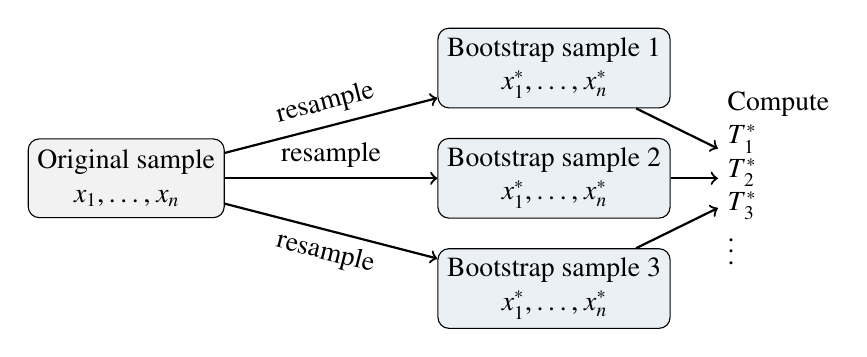
\begin{tikzpicture}[node distance=1.2cm]
\tikzstyle{box}=[draw, rounded corners, align=center, minimum width=2.4cm, minimum height=1.0cm]
\node[box, fill=gray!10] (sample) {Original sample\\$x_1,\ldots,x_n$};
\node[box, fill=oiB!10, right=2.7cm of sample, yshift=1.4cm] (b1) {Bootstrap sample 1\\$x^*_{1},\ldots,x^*_{n}$};
\node[box, fill=oiB!10, right=2.7cm of sample] (b2) {Bootstrap sample 2\\$x^*_{1},\ldots,x^*_{n}$};
\node[box, fill=oiB!10, right=2.7cm of sample, yshift=-1.4cm] (b3) {Bootstrap sample 3\\$x^*_{1},\ldots,x^*_{n}$};
\draw[->, thick] (sample) -- node[above, sloped]{resample} (b1);
\draw[->, thick] (sample) -- node[above]{resample} (b2);
\draw[->, thick] (sample) -- node[below, sloped]{resample} (b3);
\node[right=0.6cm of b2, align=left] (stats) {Compute\\$T^*_1$\\$T^*_2$\\$T^*_3$\\$\vdots$};
\draw[->, thick] (b1) -- (stats);
\draw[->, thick] (b2) -- (stats);
\draw[->, thick] (b3) -- (stats);
\end{tikzpicture}}
\end{center}

\vspace{0.4em}
\dq{Why do we sample \textbf{with} replacement rather than without replacement?}

\end{frame}

%%%%%%%%%%%%%%%%%%%%%%%%%%%%%%%%%%%%%%%%%%%%%%%%%%%%%%%%%%%%%%%%%%%%%%%%

\begin{frame}{Bootstrap Procedure}
\textbf{Input:} sample $x_1,\dots,x_n$ and a statistic $T(\cdot)$ (mean, median, quantile, \ldots)

\begin{enumerate}
\item \textbf{Resample:} draw $x^{*(b)}_1,\dots,x^{*(b)}_n$ by sampling \emph{with replacement} from $\{x_1,\dots,x_n\}$.
\item \textbf{Recompute:} $T^{*(b)} = T(x^{*(b)}_1,\dots,x^{*(b)}_n)$.
\item Repeat for $b=1,\dots,B$ (e.g., $B=2000$).
\end{enumerate}

\textbf{Output:} the \hl{bootstrap distribution} of $T^*$: our stand-in for the sampling distribution of $T$.

\vspace{6pt}
The confidence interval is then read off this distribution (next section).
\end{frame}

%%%%%%%%%%%%%%%%%%%%%%%%%%%%%%%%%%%%%%%%%%%%%%%%%%%%%%%%%%%%%%%%%%%%%%%%

\begin{frame}
\frametitle{Activity: one hand bootstrap sample}

Suppose our observed sample is
\[
40,\quad 42,\quad 44,\quad 48,\quad 56.
\]
\app{
\begin{enumerate}
\item Write down one bootstrap sample of size $5$ by sampling \textbf{with replacement} from these five numbers.
\item Compute the mean of your bootstrap sample.
\item Compare with a neighbor: did you get the same mean? Should you have?
\item Why does this mimic repeating the study?
\end{enumerate}}

\end{frame}

%%%%%%%%%%%%%%%%%%%%%%%%%%%%%%%%%%%%%%%%%%%%%%%%%%%%%%%%%%%%%%%%%%%%%%%%

\begin{frame}
\frametitle{Activity: why your neighbor got a different answer}

The observed sample $40, 42, 44, 48, 56$ has mean $\bar{x}=46.0$. \hl{Did everyone get the same bootstrap mean --- and should they have?}

\solnbox{\small One possible resample is $42, 42, 48, 40, 56$, with mean $45.6$. Your neighbor's will differ --- and that \emph{disagreement between resamples} is the entire point. It is a stand-in for the disagreement we would see between repeated studies, which is exactly the quantity a confidence interval needs.}

\vspace{0.3em}
Sampling \textbf{with} replacement lets each resample differ while keeping $n$ fixed; sampling \emph{without} it would return the same five numbers every time.

\end{frame}

%%%%%%%%%%%%%%%%%%%%%%%%%%%%%%%%%%%%%%%%%%%%%%%%%%%%%%%%%%%%%%%%%%%%%%%%
\section{From bootstrap distribution to a confidence interval}
%%%%%%%%%%%%%%%%%%%%%%%%%%%%%%%%%%%%%%%%%%%%%%%%%%%%%%%%%%%%%%%%%%%%%%%%
\begin{frame}
\frametitle{Example: bootstrap CI for the mean weight}

\begin{enumerate}
\item Compute the observed statistic:
\[
\hat{\mu}=\bar{x}=\frac{1}{n}\sum_{i=1}^n x_i.
\]
\item Resample $n$ weights with replacement from the observed weights.
\item Compute the mean of the resample.
\item Repeat many times to get $\hat{\mu}^{*(1)},\ldots,\hat{\mu}^{*(B)}$.
\item Take the 2.5th and 97.5th percentiles of the bootstrap means.
\end{enumerate}

\vspace{0.3em}
\dq{What would change if the scientific question asked for the median instead of the mean?}

\end{frame}

%%%%%%%%%%%%%%%%%%%%%%%%%%%%%%%%%%%%%%%%%%%%%%%%%%%%%%%%%%%%%%%%%%%%%%%%
\begin{frame}
\frametitle{Bootstrap distribution of the mean (kangaroo rat weight)}

\begin{center}
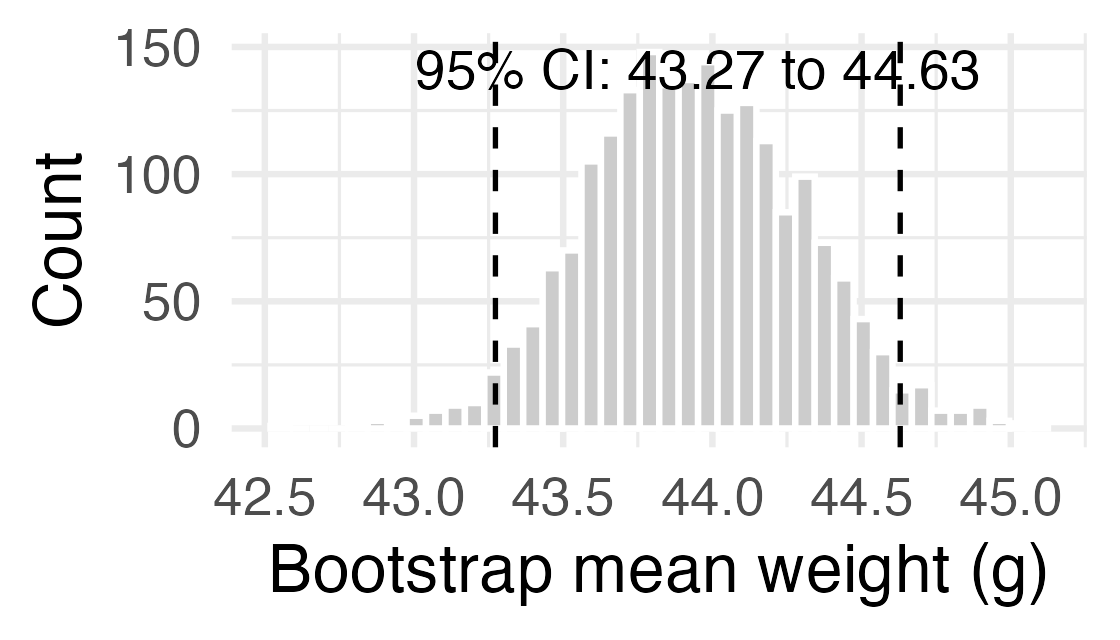
\includegraphics[width=0.55\textwidth]{dm1999_boot_mean.png}
\end{center}

\vspace{-0.5em}
\begin{itemize}
\item each bar counts bootstrap resamples ($B=2000$), \emph{not} individual rats;
\item the center sits at the observed $\bar{x}=43.95$; the spread approximates sampling variability;
\item the shaded middle 95\% is the percentile CI: $\;\hl{[43.3,\;44.6]}$ grams.
\end{itemize}

\end{frame}

%%%%%%%%%%%%%%%%%%%%%%%%%%%%%%%%%%%%%%%%%%%%%%%%%%%%%%%%%%%%%%%%%%%%%%%%
\begin{frame}
\frametitle{From bootstrap distribution to confidence interval}

After many resamples, suppose we have bootstrap statistics
\[
T^{*(1)}, T^{*(2)}, \ldots, T^{*(B)}.
\]
\vspace{0.4em}
\formula{Bootstrap percentile CI (95\%)}{
\[
\left[\text{2.5th percentile of } T^*,\quad
\text{97.5th percentile of } T^*\right].
\]}

\vspace{0.4em}
\begin{itemize}
\item This method uses the middle 95\% of the bootstrap distribution.
\item It is simple and works for many statistics, including medians and percentiles.
\end{itemize}

\end{frame}

%%%%%%%%%%%%%%%%%%%%%%%%%%%%%%%%%%%%%%%%%%%%%%%%%%%%%%%%%%%%%%%%%%%%%%%%
\begin{frame}
\frametitle{A second recipe: the standard error method}

The spread of the bootstrap distribution has a name, and it gives us the ``$\pm$'' we were missing on the very first slide.

\vspace{0.3em}
\formula{Bootstrap standard error}{
Write $\theta$ for whatever parameter we are after and $\hat{\theta}$ for the estimate computed from our sample (here $\theta=\mu$ and $\hat{\theta}=\bar{x}=43.95$). Then $\mathrm{SE}_{boot}$ is the \emph{standard deviation of the bootstrap statistics} $T^{*(1)},\ldots,T^{*(B)}$: how far a typical sample's estimate lands from the center.
\vspace{-0.2em}
\[
\text{95\% CI} \;\approx\; \hat{\theta} \;\pm\; 2\,\mathrm{SE}_{boot}
\]}

\vspace{0.3em}
This is the ``point estimate $\pm$ margin of error'' form: the margin of error is $2\,\mathrm{SE}_{boot}$.

\end{frame}

%%%%%%%%%%%%%%%%%%%%%%%%%%%%%%%%%%%%%%%%%%%%%%%%%%%%%%%%%%%%%%%%%%%%%%%%
\begin{frame}
\frametitle{Percentile or standard error?}

For the kangaroo rats the 2000 bootstrap means had $\mathrm{SE}_{boot}=0.355$ g, so the two recipes give

\vspace{-0.2em}
\begin{center}
\begin{tabular}{ll}
\toprule
Percentile method & $[43.27,\;44.63]$ \\
Standard error method & $43.95 \pm 2(0.355) = [43.24,\;44.65]$ \\
\bottomrule
\end{tabular}
\end{center}

\vspace{0.1em}
They agree to within a rounding error, because the bootstrap distribution of $\bar{x}$ is symmetric.

\vspace{0.1em}
\caution[-- when they disagree]{Not automatic. When the bootstrap distribution is skewed (medians, extreme percentiles, small $n$), \emph{trust the percentile interval}: $\pm\,2\,\mathrm{SE}$ assumes a symmetry that is not there.}

\end{frame}

%%%%%%%%%%%%%%%%%%%%%%%%%%%%%%%%%%%%%%%%%%%%%%%%%%%%%%%%%%%%%%%%%%%%%%%%
\begin{frame}[fragile]
\frametitle{Doing it in R: the bootstrap in four lines}

\begin{lstlisting}[language=R, basicstyle=\ttfamily\scriptsize]
w <- dm_1999$weight             # n = 348
mean(w)                         #> 43.95

# one resample: same size, with replacement
mean(sample(w, replace = TRUE)) #> 43.74

boot_means <- replicate(2000,   # repeat B times
  mean(sample(w, replace = TRUE)))

quantile(boot_means, c(0.025, 0.975))
#>  2.5% 97.5%
#> 43.27 44.63
\end{lstlisting}

\vspace{-0.4em}
The code \emph{is} the three steps: \hl{resample}, \hl{recompute}, \hl{repeat}, then read off the percentiles.

\end{frame}

%%%%%%%%%%%%%%%%%%%%%%%%%%%%%%%%%%%%%%%%%%%%%%%%%%%%%%%%%%%%%%%%%%%%%%%%
\begin{frame}[fragile]
\frametitle{Doing it in R: the same thing with \texttt{infer}}

\begin{lstlisting}[language=R, basicstyle=\ttfamily\small]
library(infer)

boot_dist <- dm_1999 |>
  specify(response = weight) |>
  generate(reps = 2000, type = "bootstrap") |>
  calculate(stat = "mean")

boot_dist |>
  get_confidence_interval(level = 0.95,
                          type = "percentile")
#> lower_ci upper_ci
#>    43.27    44.63
\end{lstlisting}

\vspace{-0.4em}
Same interval, same three steps, but now each step has a name.

\end{frame}

%%%%%%%%%%%%%%%%%%%%%%%%%%%%%%%%%%%%%%%%%%%%%%%%%%%%%%%%%%%%%%%%%%%%%%%%
\begin{frame}
\frametitle{The \texttt{infer} vocabulary}

\begin{center}\small
\begin{tabular}{ll}
\toprule
Step & What it does \\
\midrule
\texttt{specify()} & name the response variable \\
\texttt{generate(type = "bootstrap")} & resample with replacement \\
\texttt{calculate(stat = "mean")} & recompute the statistic \\
\texttt{get\_confidence\_interval()} & take the percentiles \\
\bottomrule
\end{tabular}
\end{center}

\vspace{0.5em}
The same four verbs will come back for randomization tests (with \texttt{type = "permute"} and a \texttt{hypothesize()} step), which is the point of learning the vocabulary rather than the individual recipe.

\end{frame}

%%%%%%%%%%%%%%%%%%%%%%%%%%%%%%%%%%%%%%%%%%%%%%%%%%%%%%%%%%%%%%%%%%%%%%%%
\begin{frame}[fragile]
\frametitle{Activity: change the question, change the statistic}

\vspace{-0.2em}
\begin{lstlisting}[language=R]
boot_dist <- dm_1999 |>
  specify(response = weight) |>
  generate(reps = 2000, type = "bootstrap") |>
  calculate(stat = "mean")
\end{lstlisting}

\vspace{-0.2em}
\app{%
Which line changes for each question below --- and to what?
\begin{enumerate}
\item How heavy is the \textbf{typical individual} rat?
\item How big are the \textbf{big ones} (the 90th percentile)?
\item What \textbf{fraction} of rats weigh more than 50 g?
\end{enumerate}}

\end{frame}

%%%%%%%%%%%%%%%%%%%%%%%%%%%%%%%%%%%%%%%%%%%%%%%%%%%%%%%%%%%%%%%%%%%%%%%%
\begin{frame}[fragile]
\frametitle{Activity: change the statistic --- solution}

{\small Recall the three questions: \textbf{(1)} the typical individual, \textbf{(2)} the 90th percentile, \textbf{(3)} the fraction heavier than 50 g.}

\solnbox{\small \textbf{(1) Median:} \texttt{calculate(stat = "median")} (one word). \textbf{(2) 90th percentile:} \texttt{calculate()} has no quantile option, so replace it with \texttt{summarise(stat = quantile(weight, 0.9))}. \textbf{(3) Proportion:} the \emph{response} itself must become binary first --- \texttt{mutate(heavy = weight > 50)}, then \texttt{specify(response = heavy, success = "TRUE")} and \texttt{calculate(stat = "prop")}.}

\vspace{0.2em}
{\small The pattern: the question names a parameter, which dictates the statistic --- \emph{one line} of code. Resample, recompute, repeat never changes.}

\end{frame}

%%%%%%%%%%%%%%%%%%%%%%%%%%%%%%%%%%%%%%%%%%%%%%%%%%%%%%%%%%%%%%%%%%%%%%%%
\section{How wide is the interval?}
%%%%%%%%%%%%%%%%%%%%%%%%%%%%%%%%%%%%%%%%%%%%%%%%%%%%%%%%%%%%%%%%%%%%%%%%
\begin{frame}
\frametitle{Choosing the confidence level}

Nothing forces us to use 95\%. The level says how much of the bootstrap distribution we keep --- a dial we set \emph{before} seeing the answer.

\vspace{-0.3em}
\begin{center}
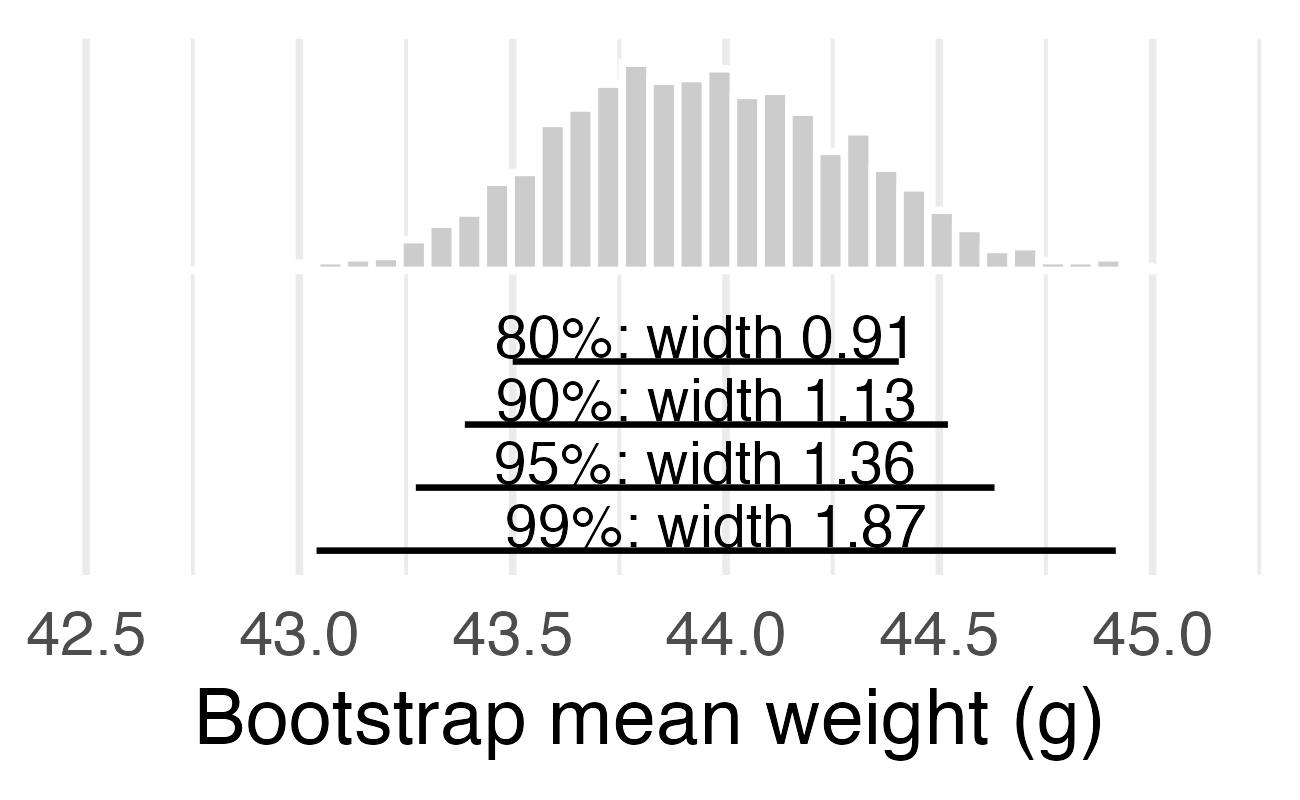
\includegraphics[width=0.50\textwidth]{ci_levels.png}
\end{center}

\vspace{-0.6em}
\dq{A 100\% confidence interval would be $(-\infty,\infty)$. What does that tell you about the price of confidence?}

\end{frame}

%%%%%%%%%%%%%%%%%%%%%%%%%%%%%%%%%%%%%%%%%%%%%%%%%%%%%%%%%%%%%%%%%%%%%%%%
\begin{frame}
\frametitle{What makes an interval narrow: the sample size}

\begin{center}
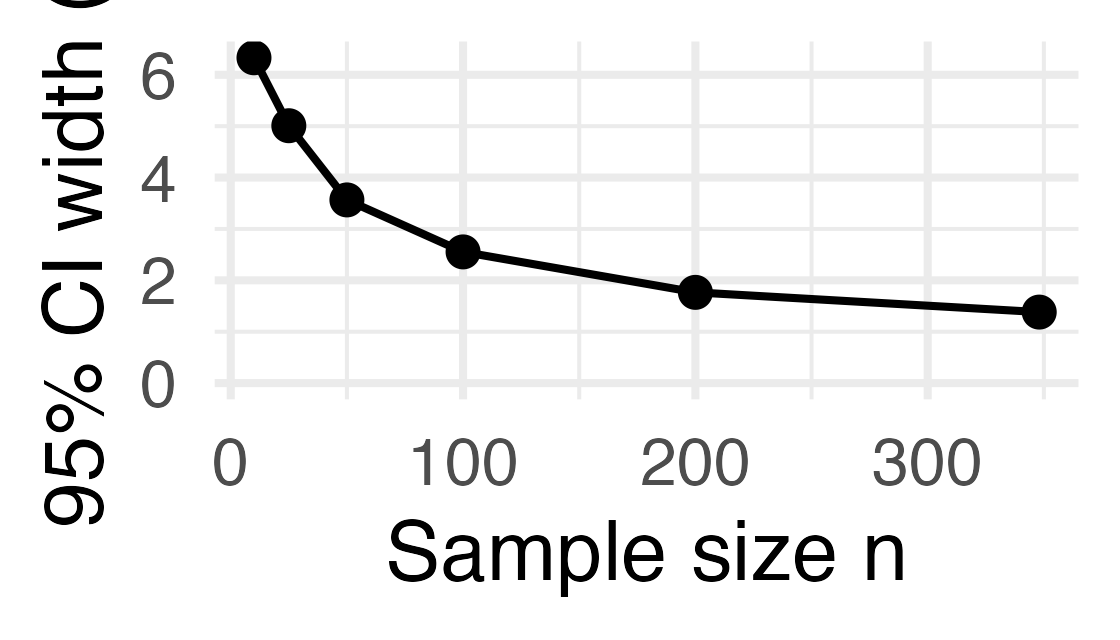
\includegraphics[width=0.62\textwidth]{width_vs_n.png}
\end{center}

\vspace{-0.3em}
\hl{$n$ is the only thing that buys precision.} More data means less sampling variability, so the bootstrap statistics cluster more tightly and the interval shrinks. Note the shape: quadrupling $n$ roughly halves the width, so precision gets expensive fast.

\end{frame}

%%%%%%%%%%%%%%%%%%%%%%%%%%%%%%%%%%%%%%%%%%%%%%%%%%%%%%%%%%%%%%%%%%%%%%%%
\begin{frame}
\frametitle{\ldots and what does \emph{not}: the number of resamples}

\begin{center}
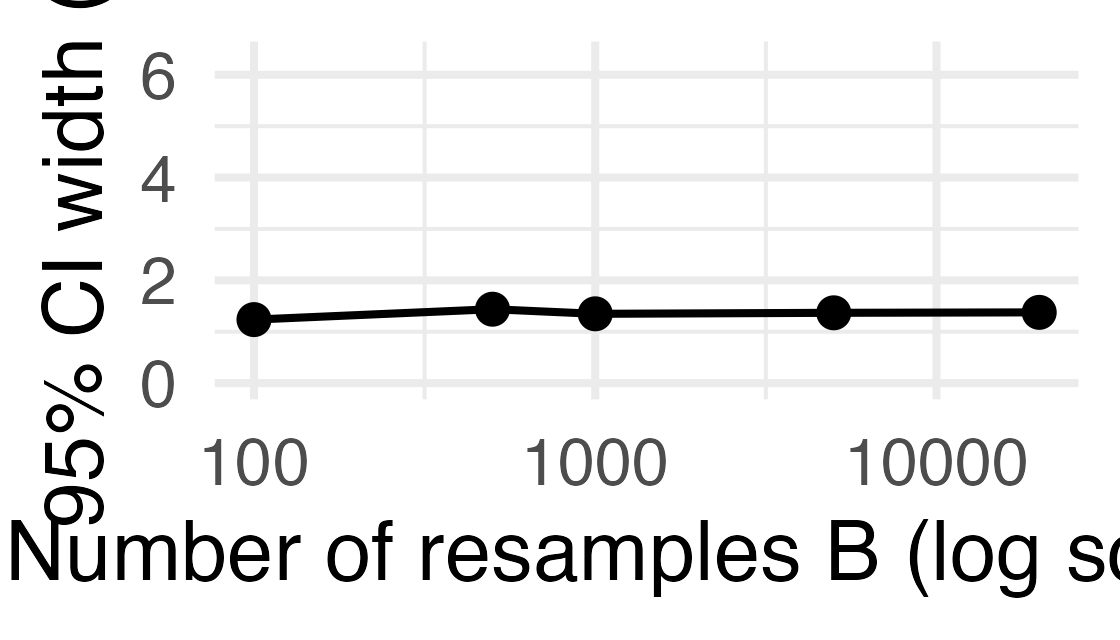
\includegraphics[width=0.62\textwidth]{width_vs_B.png}
\end{center}

\vspace{-0.3em}
\caution{Raising $B$ only reduces the \emph{simulation} noise in our estimate of the interval, so it adds no information about the rats and the width does not budge. You cannot buy precision with CPU time; if it seems to work, the code is wrong. ($B=2000$ is plenty.)}

\end{frame}

%%%%%%%%%%%%%%%%%%%%%%%%%%%%%%%%%%%%%%%%%%%%%%%%%%%%%%%%%%%%%%%%%%%%%%%%
\section{Interpreting a confidence interval}
%%%%%%%%%%%%%%%%%%%%%%%%%%%%%%%%%%%%%%%%%%%%%%%%%%%%%%%%%%%%%%%%%%%%%%%%
\begin{frame}
\frametitle{Interpreting a confidence interval}

A 95\% confidence interval is a statement about the \textbf{procedure}.

\vspace{0.4em}
\formula{What ``95\% confident'' means}{
If we repeatedly sampled from the same population and built an interval the same way each time, about 95\% of those intervals would contain the true parameter.
}

\end{frame}

%%%%%%%%%%%%%%%%%%%%%%%%%%%%%%%%%%%%%%%%%%%%%%%%%%%%%%%%%%%%%%%%%%%%%%%%
\begin{frame}{Seeing it: 20 intervals from 20 different samples}
Repeat the whole data-collection process many times, building a CI the same way each time. Here the level is \hl{80\%} --- low enough that the misses are frequent enough to see.

\vspace{-0.2em}
\begin{center}
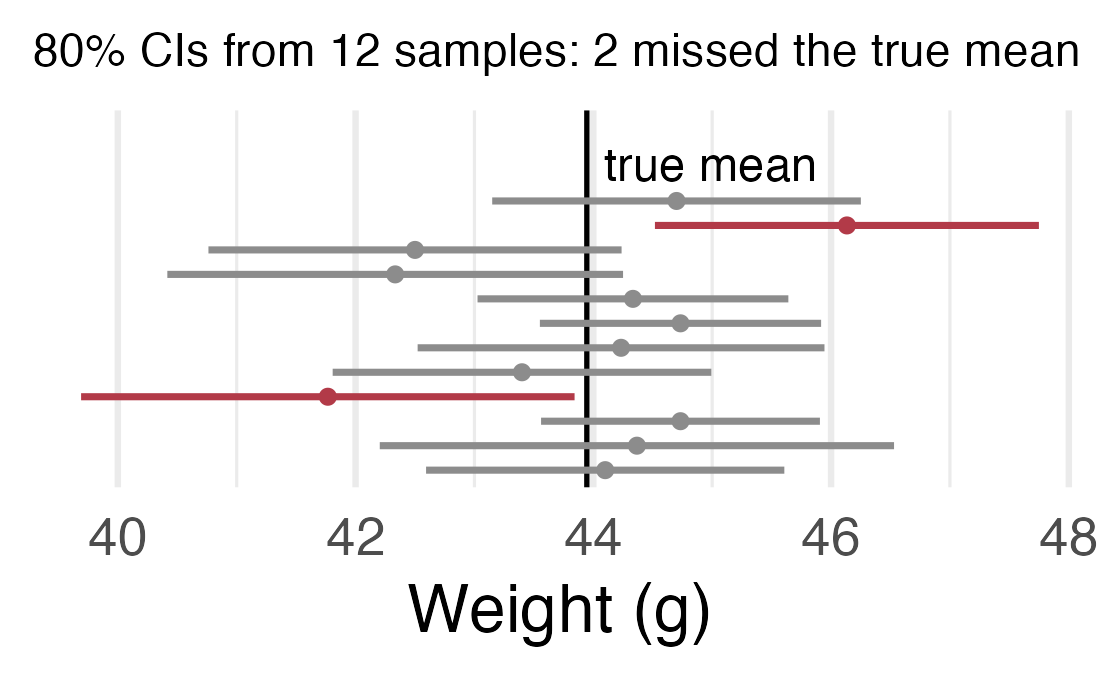
\includegraphics[width=0.55\textwidth]{ci_cartoon.png}
\end{center}

\vspace{-0.4em}
The true value (vertical line) is fixed. It is the \emph{intervals} that jump around, and about one in five of them misses.

\end{frame}

%%%%%%%%%%%%%%%%%%%%%%%%%%%%%%%%%%%%%%%%%%%%%%%%%%%%%%%%%%%%%%%%%%%%%%%%

\begin{frame}
\frametitle{What a confidence interval is not}

Common incorrect interpretations:

\begin{itemize}
\item ``There is a 95\% chance that $\mu$ is in this interval.''
  \begin{itemize}
  \item In frequentist inference, $\mu$ is fixed and the interval is random.
  \end{itemize}
\item ``95\% of the data are in this interval.''
  \begin{itemize}
  \item A CI is about the parameter, not individual observations.
  \end{itemize}
\item ``The interval proves the true value is inside.''
  \begin{itemize}
  \item It is a plausible range from a method with long-run coverage.
  \end{itemize}
\end{itemize}

\end{frame}

%%%%%%%%%%%%%%%%%%%%%%%%%%%%%%%%%%%%%%%%%%%%%%%%%%%%%%%%%%%%%%%%%%%%%%%%

\begin{frame}
\frametitle{Activity: interpret the interval}

Our 95\% bootstrap CI for the mean kangaroo rat weight was $[43.3,\;44.6]$ grams.

\app{\small
Which reading is right, and what is wrong with each of the others?
\begin{enumerate}\setlength{\itemsep}{1pt}
\item There is a 95\% probability that the mean weight is between 43.3 and 44.6 g.
\item About 95\% of kangaroo rats weigh between 43.3 and 44.6 g.
\item Using this method, repeated samples would give intervals containing the true mean about 95\% of the time.
\item The sample mean must be exactly halfway between 43.3 and 44.6 g.
\end{enumerate}}

\end{frame}

%%%%%%%%%%%%%%%%%%%%%%%%%%%%%%%%%%%%%%%%%%%%%%%%%%%%%%%%%%%%%%%%%%%%%%%%

\begin{frame}
\frametitle{Activity: interpret the interval --- solution}

\solnbox{\textbf{(3) is the only correct reading.} The other three are the three classic errors:}

\vspace{-0.3em}
{\footnotesize
\begin{itemize}\setlength{\itemsep}{1pt}
\item \textbf{(1) ``95\% probability that $\mu$ is in it.''} \soln{treats $\mu$ as random. In frequentist inference $\mu$ is fixed; it is the \emph{interval} that jumps from sample to sample.}
\item \textbf{(2) ``95\% of the rats weigh 43.3--44.6 g.''} \soln{that describes individual rats, not the parameter. 95\% of the rats we caught weigh 26--55 g, far wider.}
\item \textbf{(4) ``$\bar{x}$ is exactly halfway.''} \soln{not guaranteed. A percentile interval is read off the bootstrap distribution; if that is skewed, it is not symmetric about $\bar{x}$.}
\end{itemize}}

\end{frame}

%%%%%%%%%%%%%%%%%%%%%%%%%%%%%%%%%%%%%%%%%%%%%%%%%%%%%%%%%%%%%%%%%%%%%%%%
\section{The bootstrap in context}
%%%%%%%%%%%%%%%%%%%%%%%%%%%%%%%%%%%%%%%%%%%%%%%%%%%%%%%%%%%%%%%%%%%%%%%%
\begin{frame}
\frametitle{Three ways to get a sampling distribution}

{\scriptsize
\begin{center}
\begin{tabular}{p{0.14\textwidth}p{0.23\textwidth}p{0.23\textwidth}p{0.24\textwidth}}
\toprule
& \textbf{Randomization test} \newline (Lecture 8) & \textbf{Bootstrap CI} \newline (today) & \textbf{Mathematical model} \newline (Lecture 10) \\
\midrule
Starts from & a null hypothesis & the observed sample & a probability model + theory \\
Builds & a \hl{null} distribution & a \hl{sampling} distribution & a \emph{formula} for the sampling distribution \\
Gives you & a p-value & a confidence interval & either one, instantly \\
Answers & ``is there an effect?'' & ``how big is it?'' & both \\
Costs & simulation & simulation & assumptions (the CLT) \\
\bottomrule
\end{tabular}
\end{center}}

\vspace{0.2em}
\dq{Both resample on a computer. What is different about the \emph{world} each one simulates --- and why can a randomization test never hand you a confidence interval?}

\end{frame}

%%%%%%%%%%%%%%%%%%%%%%%%%%%%%%%%%%%%%%%%%%%%%%%%%%%%%%%%%%%%%%%%%%%%%%%%

\begin{frame}
\frametitle{Confidence intervals and tests are connected}

For many two-sided problems:

\formula{The duality}{
If a 95\% CI does not contain the null value, a two-sided test at $\alpha=0.05$ will usually reject that null.
}

\vspace{0.4em}
Example for a mean:
\begin{itemize}
\item Null hypothesis: $H_0: \mu = 40$ grams.
\item Bootstrap 95\% CI: $[43.3,\;44.6]$.
\item Since $40$ is not in the interval, this is evidence against $H_0$; and, unlike a p-value, the interval also tells us the mean is plausibly $3$ to $5$ g above $40$, the part an ecologist actually cares about.
\end{itemize}

\end{frame}

%%%%%%%%%%%%%%%%%%%%%%%%%%%%%%%%%%%%%%%%%%%%%%%%%%%%%%%%%%%%%%%%%%%%%%%%

\begin{frame}
\frametitle{The bootstrap cannot rescue a tiny sample}

\keyidea{Resampling only rearranges the data you already have. It \textbf{generates no new information} --- so it cannot fix a sample that was too small, or drawn from the wrong population.}

\vspace{-0.2em}
\begin{center}
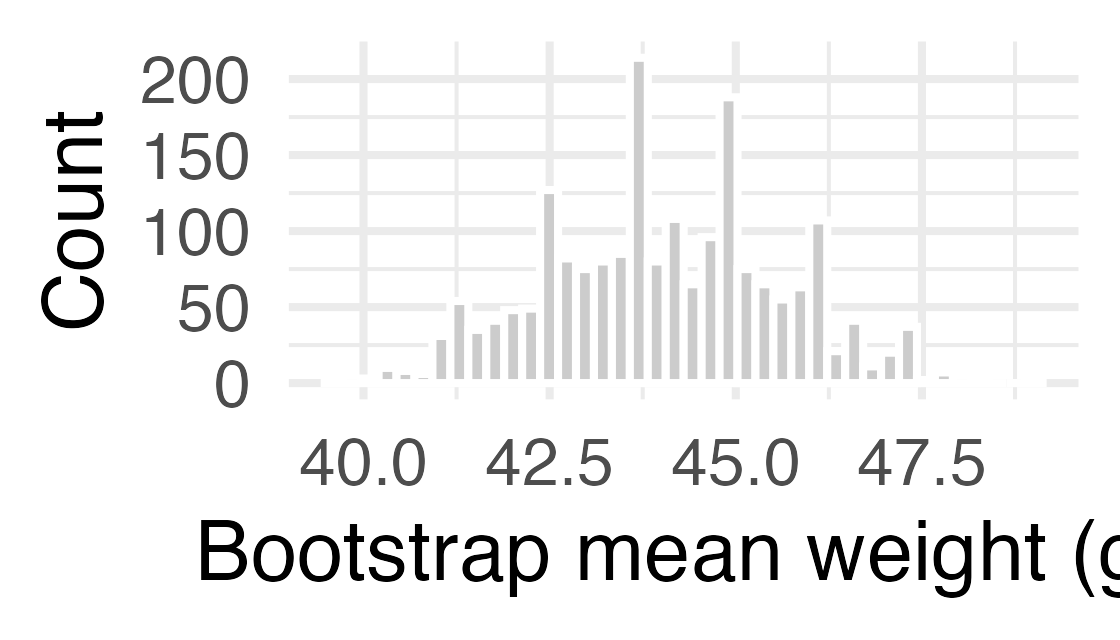
\includegraphics[width=0.42\textwidth]{boot_small_n5.png}
\end{center}

\vspace{-0.4em}
With $n=5$, every resample reuses the same five numbers, so the bootstrap distribution is lumpy and the interval simply inherits whatever those five rats happened to weigh.

\end{frame}

%%%%%%%%%%%%%%%%%%%%%%%%%%%%%%%%%%%%%%%%%%%%%%%%%%%%%%%%%%%%%%%%%%%%%%%%
\begin{frame}
\frametitle{\ldots and it fails outright for extreme statistics}

\begin{center}
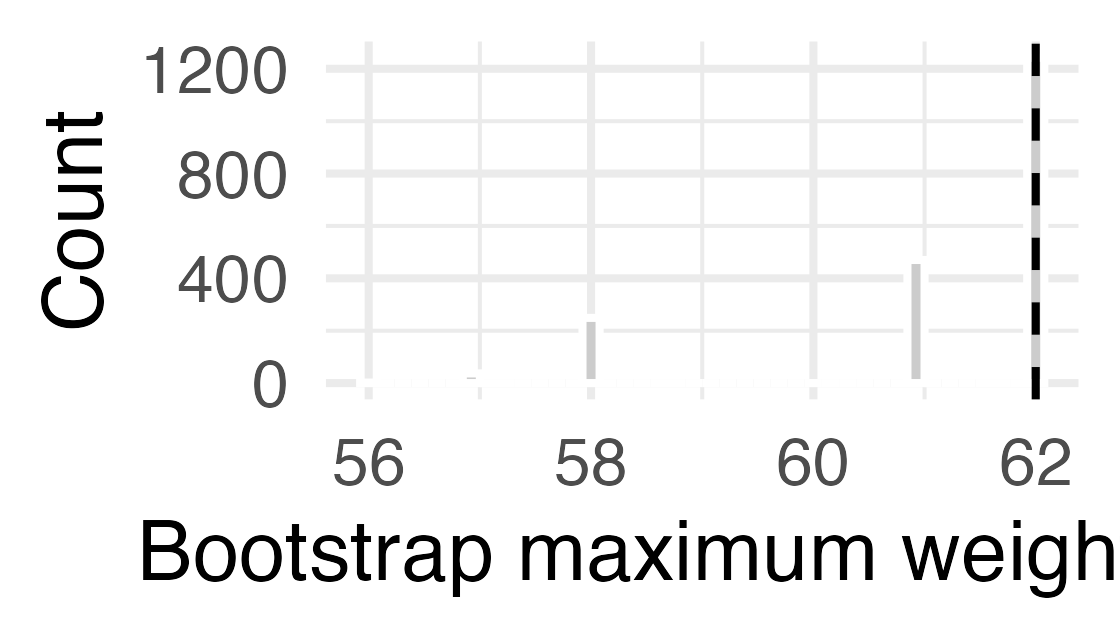
\includegraphics[width=0.42\textwidth]{boot_max.png}
\end{center}

\vspace{-0.3em}
The heaviest rat we caught weighed 62 g. \hl{No resample can ever exceed that}, so the bootstrap distribution of the maximum piles up against the dashed line, stuck below the true population maximum whatever $B$ is.

\vspace{0.2em}
\dq{The mean was fine and the maximum is hopeless. What is different about the two statistics?}

\end{frame}

%%%%%%%%%%%%%%%%%%%%%%%%%%%%%%%%%%%%%%%%%%%%%%%%%%%%%%%%%%%%%%%%%%%%%%%%

\begin{frame}
\frametitle{When is the bootstrap reasonable?}

Bootstrapping works well when:
{\small
\begin{itemize}
\item observations are independent, or the resampling respects the design;
\item the sample is representative of the population we want to talk about;
\item $n$ is large enough to carry information about the population's shape;
\item the statistic is a stable summary --- mean, median, percentile; not an extreme.
\end{itemize}}

\vspace{0.2em}
\caution{The bootstrap does \textbf{not} fix biased sampling or a badly chosen statistic. If all 348 rats were caught at one unusually lush site, every bootstrap interval will be confidently wrong.}

\end{frame}

%%%%%%%%%%%%%%%%%%%%%%%%%%%%%%%%%%%%%%%%%%%%%%%%%%%%%%%%%%%%%%%%%%%%%%%%

\begin{frame}
\frametitle{Activity: choose the inference method}

For each question, choose a randomization test, a bootstrap CI, or a mathematical model.

\app{
\begin{enumerate}
\item We want a plausible range for the mean kangaroo rat weight.
\item We want evidence that two treatments have different average outcomes.
\item We want an exact probability for the number of successes in 20 Bernoulli trials.
\item We want a plausible range for a median, whose sampling distribution is hard to derive by hand.
\end{enumerate}}

\end{frame}

%%%%%%%%%%%%%%%%%%%%%%%%%%%%%%%%%%%%%%%%%%%%%%%%%%%%%%%%%%%%%%%%%%%%%%%%

\begin{frame}
\frametitle{Activity: choose the inference method --- solution}

{\small Recall: \textbf{(1)} a range for the mean weight, \textbf{(2)} evidence that two treatments differ, \textbf{(3)} an exact binomial probability, \textbf{(4)} a range for a median.}

\solnbox{\small (1) \textbf{bootstrap CI} --- estimation, with no null in sight.
(2) \textbf{randomization test} --- a yes/no question against a null of ``no difference''.
(3) \textbf{mathematical model} --- the binomial gives the answer exactly, so simulating would only add noise.
(4) \textbf{bootstrap CI} --- estimation again, and the bootstrap does not care that the median has no tidy formula.}

\vspace{0.2em}
{\small Read what the question \emph{asks for}: a verdict against a null $\Rightarrow$ a test; a range of plausible values $\Rightarrow$ an interval; a formula whose conditions hold $\Rightarrow$ use it.}

\end{frame}

%%%%%%%%%%%%%%%%%%%%%%%%%%%%%%%%%%%%%%%%%%%%%%%%%%%%%%%%%%%%%%%%%%%%%%%%
\section{Wrap-up}
%%%%%%%%%%%%%%%%%%%%%%%%%%%%%%%%%%%%%%%%%%%%%%%%%%%%%%%%%%%%%%%%%%%%%%%%
\begin{frame}
\frametitle{Summary}

\begin{itemize}
\item A confidence interval gives a plausible \emph{range} for a parameter: estimate $\pm$ uncertainty.
\item Bootstrapping approximates repeated sampling by \hl{resampling your own data with replacement}: resample, recompute, repeat.
\item The bootstrap distribution is a distribution of a \emph{statistic}. Its center is $\hat\theta$; what we use is its \emph{spread}.
\item Two recipes --- the \hl{percentile} interval, and $\hat\theta \pm 2\,\mathrm{SE}_{boot}$. They agree when the distribution is symmetric.
\item ``95\% confident'' describes the \emph{procedure's} long-run coverage, not this one interval.
\item Only $n$ narrows an interval; $B$ does not, and no amount of resampling rescues a bad sample.
\end{itemize}

\end{frame}





\end{document}
